\documentclass[12pt]{beamer}
\usepackage{../Estilos/BeamerFC}
\usepackage{../Estilos/ColoresLatex}
\usepackage{courier}
\usepackage{listingsutf8}
\usepackage{listings}
\usepackage{xcolor}
\usepackage{textcomp}
\usepackage{color}
\definecolor{deepblue}{rgb}{0,0,0.5}
\definecolor{brown}{rgb}{0.59, 0.29, 0.0}
\definecolor{OliveGreen}{rgb}{0,0.25,0}
% \usepackage{minted}

\DeclareCaptionFont{white}{\color{white}}
\DeclareCaptionFormat{listing}{\colorbox{gray}{\parbox{0.98\textwidth}{#1#2#3}}}
\captionsetup[lstlisting]{format=listing,labelfont=white,textfont=white}
\renewcommand{\lstlistingname}{Código}


\definecolor{Code}{rgb}{0,0,0}
\definecolor{Keywords}{rgb}{255,0,0}
\definecolor{Strings}{rgb}{255,0,255}
\definecolor{Comments}{rgb}{0,0,255}
\definecolor{Numbers}{rgb}{255,128,0}

\makeatletter

\newif\iffirstchar\firstchartrue
\newif\ifstartedbyadigit
\newif\ifprecededbyequalsign

\newcommand\processletter
{%
  \ifnum\lst@mode=\lst@Pmode%
    \iffirstchar%
        \global\startedbyadigitfalse%
      \fi
      \global\firstcharfalse%
    \fi
}

\newcommand\processdigit
{%
  \ifnum\lst@mode=\lst@Pmode%
      \iffirstchar%
        \global\startedbyadigittrue%
      \fi
      \global\firstcharfalse%
  \fi
}

\lst@AddToHook{OutputOther}%
{%
  \lst@IfLastOtherOneOf{=}
    {\global\precededbyequalsigntrue}
    {}%
}

\lst@AddToHook{Output}%
{%
  \ifprecededbyequalsign%
      \ifstartedbyadigit%
        \def\lst@thestyle{\color{orange}}%
      \fi
    \fi
  \global\firstchartrue%
  \global\startedbyadigitfalse%
  \global\precededbyequalsignfalse%
}

\lstset{ 
language=Python,                % choose the language of the code
basicstyle=\footnotesize\ttfamily,       % the size of the fonts that are used for the code
numbers=left,                   % where to put the line-numbers
numberstyle=\scriptsize,      % the size of the fonts that are used for the line-numbers
stepnumber=1,                   % the step between two line-numbers. If it is 1 each line will be numbered
numbersep=5pt,                  % how far the line-numbers are from the code
backgroundcolor=\color{white},  % choose the background color. You must add \usepackage{color}
showspaces=false,               % show spaces adding particular underscores
showstringspaces=false,         % underline spaces within strings
showtabs=false,                 % show tabs within strings adding particular underscores
frame=single,   		% adds a frame around the code
tabsize=2,  		% sets default tabsize to 2 spaces
captionpos=t,   		% sets the caption-position to bottom
breaklines=true,    	% sets automatic line breaking
breakatwhitespace=false,    % sets if automatic breaks should only happen at whitespace
escapeinside={| |},  % if you want to add a comment within your code
stringstyle =\color{OliveGreen},
otherkeywords={as, np.array, np.concatenate, np.linspace, linspace, interpolate.interp1d, kind, plt.plot, .copy, np.arange, np.cos, np.pi, lw, ls, label, splrep, splev, plt.legend, loc, plt.title, plt.ylim, plt.show, sign, math.ceil, math.log, np.sqrt, np.exp, np.zeros, plt.xlabel, plt.ylabel, plt.xlim, np.identity, random, np.dot, np.outer, np.diagonal },             % Add keywords here
keywordstyle = \color{blue},
commentstyle = \color{darkcerulean},
identifierstyle = \color{black},
literate=%
         {á}{{\'a}}1
         {é}{{\'e}}1
         {í}{{\'i}}1
         {ó}{{\'o}}1
         {ú}{{\'u}}1
%
%keywordstyle=\ttb\color{deepblue}
%fancyvrb = true,
}

\lstdefinestyle{FormattedNumber}{%
    literate={0}{{\textcolor{red}{0}}}{1}%
             {1}{{\textcolor{red}{1}}}{1}%
             {2}{{\textcolor{red}{2}}}{1}%
             {3}{{\textcolor{red}{3}}}{1}%
             {4}{{\textcolor{red}{4}}}{1}%
             {5}{{\textcolor{red}{5}}}{1}%
             {6}{{\textcolor{red}{6}}}{1}%
             {7}{{\textcolor{red}{7}}}{1}%
             {8}{{\textcolor{red}{8}}}{1}%
             {9}{{\textcolor{red}{9}}}{1}%
             {.0}{{\textcolor{red}{.0}}}{2}% Following is to ensure that only periods
             {.1}{{\textcolor{red}{.1}}}{2}% followed by a digit are changed.
             {.2}{{\textcolor{red}{.2}}}{2}%
             {.3}{{\textcolor{red}{.3}}}{2}%
             {.4}{{\textcolor{red}{.4}}}{2}%
             {.5}{{\textcolor{red}{.5}}}{2}%
             {.6}{{\textcolor{red}{.6}}}{2}%
             {.7}{{\textcolor{red}{.7}}}{2}%
             {.8}{{\textcolor{red}{.8}}}{2}%
             {.9}{{\textcolor{red}{.9}}}{2}%
             {\ }{{ }}{1}% handle the space
         ,%
          %mathescape=true
          escapeinside={__}
          }



\usetheme{Dresden}
\usecolortheme{seahorse}
%\useoutertheme{default}
\setbeamercovered{invisible}
% or whatever (possibly just delete it)
\setbeamertemplate{section in toc}[sections numbered]
\setbeamertemplate{subsection in toc}[subsections numbered]
\setbeamertemplate{subsection in toc}{\leavevmode\leftskip=3.2em\rlap{\hskip-2em\inserttocsectionnumber.\inserttocsubsectionnumber}\inserttocsubsection\par}
\setbeamercolor{section in toc}{fg=blue}
\setbeamercolor{subsection in toc}{fg=blue}
\setbeamercolor{frametitle}{fg=blue}
\setbeamertemplate{caption}[numbered]

\setbeamertemplate{footline}
\beamertemplatenavigationsymbolsempty
\setbeamertemplate{headline}{}

\makeatletter
\setbeamercolor{section in foot}{bg=gray!30, fg=black!90!orange}
\setbeamercolor{subsection in foot}{bg=blue!30!yellow, fg=red}
\setbeamertemplate{footline}
{
  \leavevmode%
  \hbox{%
  \begin{beamercolorbox}[wd=.333333\paperwidth,ht=2.25ex,dp=1ex,center]{section in foot}%
    \usebeamerfont{section in foot} \insertsection
  \end{beamercolorbox}}%
  \begin{beamercolorbox}[wd=.333333\paperwidth,ht=2.25ex,dp=1ex,center]{subsection in foot}%
    \usebeamerfont{subsection in foot}  \insertsubsection
  \end{beamercolorbox}%
  \begin{beamercolorbox}[wd=.333333\paperwidth,ht=2.25ex,dp=1ex,right]{date in head/foot}%
    \usebeamerfont{date in head/foot} \insertshortdate{} \hspace*{2em}
    \insertframenumber{} / \inserttotalframenumber \hspace*{2ex} 
  \end{beamercolorbox}}%
  \vskip0pt%
\makeatother 

\makeatletter
\patchcmd{\beamer@sectionintoc}{\vskip1.5em}{\vskip0.8em}{}{}
\makeatother

\usefonttheme{serif}

\title{\large{Diferenciación numérica}}
\subtitle{Tema 2 - Operaciones matemáticas básicas}
\author{M. en C. Gustavo Contreras Mayén}
\date{}

\begin{document}
\maketitle

\section*{Contenido}
\frame{\tableofcontents[currentsection, hideallsubsections]}

\section{Problema inicial}
\frame{\tableofcontents[currentsection, hideothersubsections]}
\subsection{Planteamiento}

\begin{frame}
\frametitle{Problema inicial}
Dada una función $f (x)$ y un valor $x$, queremos calcular:
\pause
\begin{align*}
\dv[n]{f (x)}{x}
\end{align*}
\end{frame}
\begin{frame}
\frametitle{Evaluando la derivada}
Usamos la diferenciación numérica para el siguiente problema: \pause se nos da una función $y = f (x)$ y deseamos obtener una de sus derivadas en el punto $x = x_{k}$.
\end{frame}
\begin{frame}
\frametitle{Sobre la función}
Cuando decimos \enquote{función dada} significa que:
\setbeamercolor{item projected}{bg=lilac,fg=white}
\setbeamertemplate{enumerate items}{%
\usebeamercolor[bg]{item projected}%
\raisebox{1.5pt}{\colorbox{bg}{\color{fg}\footnotesize\insertenumlabel}}%
}
\begin{enumerate}[<+->]
\item Tenemos un algoritmo para calcular la función, o
\item Contamos con un conjunto de puntos discretos $(x_{i}, y_{i})$, $i = 0, 1,\ldots,N$.
\end{enumerate}
\pause
En cualquier caso, tenemos acceso a un número finito de pares de datos $(x, y)$ a partir de los cuales, podemos calcular la derivada.
\end{frame}
\begin{frame}
\frametitle{La interpolación de nuevo}
Si estás pensando en que la diferenciación numérica se relaciona con interpolación, tienes toda la razón.
\\
\bigskip
\pause
Ya que es un medio para encontrar la derivada a partir de una aproximación con un polinomio, y luego diferenciar.
\end{frame}
\begin{frame}
\frametitle{Desarrollo en series de Taylor}
Una herramienta igualmente eficaz es el desarrollo en serie de Taylor de $f (x)$ sobre el punto de $x_{k}$, lo que representa como ventaja de que nos proporciona información acerca del error cometido en la aproximación.
\end{frame}
\begin{frame}
\frametitle{Cuidados con la diferenciación}
La diferenciación numérica no es un proceso particularmente exacto: \pause se presentan un conflicto entre \textcolor{ao}{los errores de redondeo} (debido a la precisión de la máquina) y \textcolor{beaver}{los errores inherentes a la interpolación}.
\\
\bigskip
\pause
Por esta razón, la derivada de una función no debe de ser calculada con la misma precisión que la propia función.
\end{frame}

\section{Aproximación por diferencias finitas}
\frame{\tableofcontents[currentsection, hideothersubsections]}
\subsection{Definición}

\begin{frame}
\frametitle{Aproximación por diferencias finitas}
La derivación por aproximación por diferencias finitas de las derivadas de $f (x)$, se basa en el desarrollo de series de Taylor hacia adelante y hacia atrás de $f (x)$ alrededor de $x$:
\pause
\begin{eqnarray*}
\begin{aligned}
f (x + h) &= f(x) + h \, \pderivada{f} (x) + \dfrac{h^{2}}{2!} \, \sderivada{f} (x) + \dfrac{h^{3}}{3!} \, \tderivada{f} (x) + \\[0.5em]
&+ \dfrac{h^{4}}{4!} \, f^{(4)} (x) + \ldots \\ \pause
f (x - h) &= f(x) - h \, \pderivada{f} (x) + \dfrac{h^{2}}{2!} \, \sderivada{f} (x) - \dfrac{h^{3}}{3!} \, \tderivada{f} (x) + \\[0.5em]
&+ \dfrac{h^{4}}{4!} \, f^{(4)}(x) - \ldots
\end{aligned}
\end{eqnarray*}
\end{frame}
\begin{frame}
\frametitle{Aproximación por diferencias finitas}
\begin{eqnarray*}
\begin{aligned}
f (x + 2 h) &= f(x) + 2 \, h \, \pderivada{f} (x) + \dfrac{(2 h)^{2}}{2!} \, \sderivada{f} (x) + \dfrac{(2 h)^{3}}{3!} \, \tderivada{f} (x) + \\[0.5em]
&+ \dfrac{(2 h)^{4}}{4!} \, f^{(4)}(x) + \ldots \\ \pause
f( x - 2 h) &= f(x) - 2 \, h \, \pderivada{f} (x) + \dfrac{(2 h)^{2}}{2!} \, \sderivada{f} (x) - \dfrac{(2 h)^{3}}{3!} \, \tderivada{f} (x) + \\[0.5em]
&+  \dfrac{(2 h)^{4}}{4!} \, f^{(4)}(x) - \ldots
\end{aligned}
\end{eqnarray*}
\end{frame}
\begin{frame}
\frametitle{Suma de las diferencias}
Si sumamos las diferencias hacia adelante y hacia atrás, se tiene que:
\pause
\begin{eqnarray*}
\begin{aligned}
f (x + h) + f (x - h) &= 2 \, f (x) + h^{2} \, \sderivada{f} (x) + \dfrac{h^{4}}{12} \, f^{(4)}(x) + \ldots \\ \pause
f (x + h) - f (x - h) &= 2 \, h \, \pderivada{f} (x) + \dfrac{h^{3}}{3} \, \tderivada{f} (x) + \ldots \\ \pause
f (x + 2 h) + f ( x - 2 h) &= 2 \, f (x) + 4 \, h^{2} \, \sderivada{f} (x) + \dfrac{4 \, h^{4}}{3} \, f^{(4)} (x) +\ldots \\ \pause
f (x + 2 h) - f (x - 2 h) &= 4 \, h \, \pderivada{f} (x) + \dfrac{8 \, h^{3}}{3} \tderivada{f} (x) + \ldots
\end{aligned}
\end{eqnarray*}
\end{frame}

\section{Técnicas de aproximación}
\frame{\tableofcontents[currentsection, hideothersubsections]}
\subsection{Diferencias centrales}

\begin{frame}
\frametitle{Aproximación por diferencias centrales}
Tomando la segunda suma de la lista anterior:
\begin{align*}
f (x + h) - f (x - h) &= 2 \, h \, \pderivada{f} (x) + \dfrac{h^{3}}{3} \, \tderivada{f} (x) + \ldots
\end{align*}
\pause
de donde despejamos $\pderivada{f} (x)$, tenemos que:
\pause
\begin{align*}
\pderivada{f} (x) = \dfrac{f( x+ h ) - f(x - h)}{2 \, h} - \dfrac{h^{2}}{6} \, \tderivada{f} (x) - \ldots
\end{align*}
\end{frame}
\begin{frame}
\frametitle{Aproximación por diferencias centrales}
Que de manera equivalente presentamos como:
\pause
\begin{align*}
\pderivada{f} (x) = \dfrac{f(x + h) - f(x - h)}{2 \, h} + \order{h^{2}}
\end{align*}
que es la llamada \textcolor{ao}{aproximación por diferencias centrales} de $\pderivada{f} (x)$.
\end{frame}
\begin{frame}
\frametitle{Diferencias centrales de orden 2}
De manera similar, de la expresión:
\pause
\begin{align*}
f (x + h) + f (x - h) &= 2 \, f (x) + h^{2} \, \sderivada{f} (x) + \dfrac{h^{4}}{12} \, f^{(4)}(x) + \ldots
\end{align*}
obtenemos la aproximación por diferencias centrales para la derivada de segundo orden $\sderivada{f} (x)$:
\pause
\begin{align*}
\sderivada{f} (x) =  \dfrac{f(x + h) - 2 \, f (x) + f (x - h)}{h^{2}} + \dfrac{h^{2}}{12} \, f^{(4)}(x) + \ldots
\end{align*}
\end{frame}
\begin{frame}
\frametitle{Diferencias centrales de orden 2}
Es decir:
\pause
\begin{align*}
\sderivada{f} (x) =  \dfrac{f(x + h) - 2 \, f (x) + f (x - h)}{h^{2}} + \order{h^{2}}
\end{align*}
\end{frame}

\subsection{Diferencias hacia adelante/atrás}

\begin{frame}
\frametitle{Aproximación por diferencias hacia adelante/atrás}
Las aproximaciones por diferencias centrales no siempre son útiles.
\\
\bigskip
\pause
Por ejemplo, considera la situación en que se da la función en los $n$ puntos discretos $x_{0}, x_{1}, \ldots,x_{n}$. \pause Dado que las diferencias centrales utilizan valores de la función en cada lado de $x$, no sería posible calcular las derivadas en $x_{0}$ y $x_{n}$.
\end{frame}
\begin{frame}
\frametitle{Aproximación por diferencias hacia adelante/atrás}
Es cierto, que necesitaremos una expresión para diferencias finitas que evalúe la función en un solo lado de $x$.
\\
\bigskip
\pause
Estas expresiones son llamadas aproximaciones por diferencias finitas \textcolor{red}{hacia adelante} y \textcolor{blue}{hacia atrás}.
\end{frame}
\begin{frame}
\frametitle{Recuperando la expresión}
Despejamos $\pderivada{f} (x)$ de:
\pause
\begin{align*}
f (x + h) &= f(x) + h \, \pderivada{f} (x) + \dfrac{h^{2}}{2!} \, \sderivada{f} (x) + \dfrac{h^{3}}{3!} \, \tderivada{f} (x) + \\[0.5em]
&+ \dfrac{h^{4}}{4!} \, f^{(4)} (x) + \ldots
\end{align*}
\pause
para obtener:
\pause
\begin{align*}
\pderivada{f} (x) = \dfrac{f (x + h) - f (x)}{h} - \dfrac{h}{2} \, \sderivada{f} (x) - \dfrac{h^{2}}{6} \, \tderivada{f} (x) - \ldots
\end{align*}
\end{frame}
\begin{frame}
\frametitle{Diferencias centrales hacia adelante}
Manteniendo los primeros términos, tenemos la \textcolor{red}{aproximación por diferencias centrales hacia adelante}:
\pause
\begin{align*}
\pderivada{f} (x) = \dfrac{f (x + h) - f (x)}{h} + \order{h}
\end{align*}
\end{frame}
\begin{frame}
\frametitle{Diferencias centrales hacia atrás}
De manera similar, con la expresión:
\begin{align*}
f (x - h) &= f(x) - h \, \pderivada{f} (x) + \dfrac{h^{2}}{2!} \, \sderivada{f} (x) - \dfrac{h^{3}}{3!} \, \tderivada{f} (x) + \\[0.5em]
&+ \dfrac{h^{4}}{4!} \, f^{(4)}(x) - \ldots
\end{align*}
\pause
Obtenemos la \textcolor{blue}{aproximación por diferencias hacia atrás}:
\pause
\begin{align*}
\pderivada{f} (x) = \dfrac{f (x) - f(x - h)}{h} + \order{h}
\end{align*}
\end{frame}
\begin{frame}
\frametitle{Diferencias centrales hacia atrás}
Hay que hacer notar que el error es $\order{h}$, no es tan bueno como $\order{h^{2}}$ en la aproximación por diferencias centrales.
\end{frame}

\subsection{2a. aprox. por diferencias centrales}

\begin{frame}
\frametitle{Segunda aproximación por diferencias centrales}
Las aproximaciones por diferencias centrales del tipo $\order{h}$ no son tan populares debido a que es más común usar expresiones del tipo $\order{h^{2}}$.
\\
\bigskip
\pause
Para obtener una fórmula con diferencias centrales con ese orden de error, tenemos que incluir más términos de la serie de Taylor.
\end{frame}
\begin{frame}
\frametitle{Más términos en la serie de Taylor}
Consideremos las siguientes expresiones:
\pause
\begin{eqnarray*}
\begin{aligned}
f (x + h) &= f (x) + h \, \pderivada{f} (x) + \dfrac{h^{2}}{2!} \, \sderivada{f} (x) + \dfrac{h^{3}}{3!} \, \tderivada{f} (x) + \\[0.5em]
&+ \dfrac{h^{4}}{4!} \, f^{(4)} (x) + \ldots \\ \pause
f (x + 2 h) &= f (x) + 2 \, h \, \pderivada{f} (x) + \dfrac{(2 h)^{2}}{2!} \, \sderivada{f} (x) + \dfrac{(2 \, h)^{3}}{3!} \tderivada{f} (x) + \\[0.5em]
&+ \dfrac{(2 \, h)^{4}}{4!} \, f^{(4)}(x) + \ldots
\end{aligned}
\end{eqnarray*}
\end{frame}
\begin{frame}
\frametitle{Más términos en la serie de Taylor}
Eliminamos $\sderivada{f} (x)$ multiplicando la primera ecuación y restándola de la segunda, para obtener:
\pause
\begin{align*}
f (x + 2 \, h) - 4 \, f (x + h) &= -3 \, f (x) - 2 \, h \, \pderivada{f} (x) + \\[0.5em]
&+ \dfrac{2 \, h^{3}}{3} \, \tderivada{f} (x) + \ldots
\end{align*}
\end{frame}
\begin{frame}
\frametitle{Simplificando la expresión}
Por lo tanto:
\pause
\begin{align*}
\pderivada{f} (x) = \dfrac{-f (x + 2 \, h) + 4 \, f(x + h) - 3 \, f (x)}{2 \, h} + \dfrac{h^{2}}{3} \, \tderivada{f} (x) + \ldots
\end{align*}
que simplificando resulta:
\pause
\begin{align*}
\pderivada{f} (x) = \dfrac{- f (x + 2 \, h) + 4 \, f (x + h) - 3 \, f (x)}{2 \, h} + \order{h^{2}}
\end{align*}
siendo la expresión para la \textcolor{byzantine}{segunda aproximación por diferencias finitas hacia adelante}.
\end{frame}

\section{Errores en las aprox. por dif. fin.}
\frame{\tableofcontents[currentsection, hideothersubsections]}
\subsection{Estudiando el error}

\begin{frame}
\frametitle{Errores en las aprox. por diferencias finitas}
El efecto del error por redondeo puede ser profundo: \pause si $h$ es muy pequeña, valores de $f(x)$, $f (x \pm h)$, $f (x \pm 2h)$, etc. serán aproximadamente iguales.
\end{frame}
\begin{frame}
\frametitle{Errores en las aprox. por diferencias finitas}
Cuando se multiplican por los coeficientes y se suman, podemos perder un número grande de términos.
\\
\bigskip
\pause
Por otro lado, no debemos de hacer muy grande el valor de $h$, ya que el error debido al truncamiento, sería excesivo.
\end{frame}
\begin{frame}
\frametitle{Reduciendo el error}
Para manejar esta situación que siempre se va a presentar, podemos apoyarnos con las siguientes opciones:
\setbeamercolor{item projected}{bg=cadmiumorange,fg=black}
\setbeamertemplate{enumerate items}{%
\usebeamercolor[bg]{item projected}%
\raisebox{1.5pt}{\colorbox{bg}{\color{fg}\footnotesize\insertenumlabel}}%
}
\begin{enumerate}[<+->]
\item Usar doble precisión.
\item Usar diferencias finitas en donde se alcance el orden de $\order{h^{2}}$.
\end{enumerate}
\end{frame}

\subsection{Ejercicio 1}

\begin{frame}
\frametitle{Hagamos un ejercicio.}
\setbeamercolor{item projected}{bg=carmine,fg=white}
\setbeamertemplate{enumerate items}{%
\usebeamercolor[bg]{item projected}%
\raisebox{1.5pt}{\colorbox{bg}{\color{fg}\footnotesize\insertenumlabel}}%
}
\begin{enumerate}[<+->]
\item Calcula la segunda derivada de $f (x) = e^{-x}$ en $x = 1$ a partir de la fórmula de diferencias centrales.
\item Comienza con $h = 0.64$, para luego calcular de nuevo la derivada pero con $h /2$, para llegar a $h = 0.00008$.
\item Calcula el error relativo en cada paso, el valor exacto es $\sderivada{f} (1) = \exp(-1) = 0.36787944$
\end{enumerate}
\end{frame}
\begin{frame}
\frametitle{Suposiciones importantes}
Toma en cuenta de que las funciones para las aproximaciones por diferencias finitas deberán de estar en un módulo llamado \funcionazul{moduloDiferencias}.
\\
\bigskip
\pause
Además, la función \funcionazul{error\_rel} también se debe de llamar preferentemente de otro módulo, recuerda que los módulo permiten reutilizar código sin necesidad de copiar en otros módulos la misma función.
\end{frame}
\begin{frame}[allowframebreaks, fragile]
\frametitle{Implementando el código}
\begin{lstlisting}[caption=Código para obtener la aproximación de la segunda derivada]
from moduloDiferencias import ddif_central
from math import exp

def funcion(x):
    return exp(-x)

h = 0.64
x = 1.
exacta = 0.36787944

for i in range(1, 15):
    aproximacion = ddif_central(funcion, x, h)
    print('{0:1.5f} \t {1:1.6f} \t {2:1.5e}'.format(h, aproximacion, error_rel(exacta, aproximacion))
    h = h*0.5
\end{lstlisting}
\end{frame}
\begin{frame}
\frametitle{Valores obtenidos}
\begin{table}
\renewcommand{\arraystretch}{0.9}
\centering
\begin{tabular}{c c c}
h & derivada & error \\ \hline
$0.64000$ & $0.38060910$ & $1.272966e-02$ \\ \hline
$0.32000$ & $0.37102941$ & $3.149974e-03$ \\ \hline
$0.16000$ & $0.36866492$ & $7.854807e-04$ \\ \hline
$0.08000$ & $0.36807569$ & $1.962454e-04$ \\ \hline
\ldots & \ldots & \ldots \\ \hline
% $0.04000$ & $0.36792849$ & $4.905438e-05$ \\ \hline
% $0.02000$ & $0.36789170$ & $1.226398e-05$ \\ \hline
% $0.01000$ & $0.36788251$ & $3.066844e-06$ \\ \hline
% $0.00500$ & $0.36788021$ & $7.675879e-07$ \\ \hline
% $0.00250$ & $0.36787963$ & $1.927744e-07$ \\ \hline
% $0.00125$ & $0.36787949$ & $4.904049e-08$ \\ \hline
% $0.00063$ & $0.36787945$ & $1.305150e-08$ \\ \hline
% $0.00031$ & $0.36787944$ & $4.524988e-09$ \\ \hline
% $0.00016$ & $0.36787944$ & $1.727788e-09$ \\ \hline
% $0.00008$ & $0.36787944$ & $1.727788e-09$ \\ \hline
\end{tabular}    
\end{table}
\end{frame}
\begin{frame}
\frametitle{Valores obtenidos}
\begin{table}
\renewcommand{\arraystretch}{0.9}
\centering
\begin{tabular}{c c c}\hline
h & derivada & error \\ \hline
% $0.64000$ & $0.38060910$ & $1.272966e-02$ \\ \hline
% $0.32000$ & $0.37102941$ & $3.149974e-03$ \\ \hline
% $0.16000$ & $0.36866492$ & $7.854807e-04$ \\ \hline
% $0.08000$ & $0.36807569$ & $1.962454e-04$ \\ \hline
\ldots & \ldots & \ldots \\ \hline
% $0.04000$ & $0.36792849$ & $4.905438e-05$ \\ \hline
% $0.02000$ & $0.36789170$ & $1.226398e-05$ \\ \hline
% $0.01000$ & $0.36788251$ & $3.066844e-06$ \\ \hline
% $0.00500$ & $0.36788021$ & $7.675879e-07$ \\ \hline
% $0.00250$ & $0.36787963$ & $1.927744e-07$ \\ \hline
$0.00125$ & $0.36787949$ & $4.904049e-08$ \\ \hline
$0.00063$ & $0.36787945$ & $1.305150e-08$ \\ \hline
$0.00031$ & $0.36787944$ & $4.524988e-09$ \\ \hline
$0.00016$ & $0.36787944$ & $1.727788e-09$ \\ \hline
$0.00008$ & $0.36787944$ & $1.727788e-09$ \\ \hline
\end{tabular}    
\end{table}
\end{frame}
\begin{frame}
\frametitle{Conclusión}
El valor obtenido para la $\sderivada{f} (x)$ en $x = 1$, se alcanzó con $h = 0.00031$.
\\
\bigskip
\pause
Como se mencionó anteriormente, la diferenciación numérica es una operación donde los errores pueden devolver valores no esperados, por ello es importante estudiar los resultados con cuidado.
\end{frame}

\subsection{Ejercicio 2}

\begin{frame}
\frametitle{Hagamos un segundo ejercicio}
El siguiente arreglo tiene por dimensiones $a = \SI{100}{\milli\meter}$,  $b = \SI{120}{\milli\meter}$, $c = \SI{100}{\milli\meter}$ y $d = \SI{180}{\milli\meter}$:
\begin{center}
\begin{tikzpicture}[font=\small]
\draw (0,0) node [above left] {A} circle (0.05);
\draw (1.8,2) node [above left] {B} circle (0.05);
\draw (3.5,2.5)node [above right] {C} circle (0.05);
\draw (6,0) node [above right] {D} circle (0.05);
\draw [dashed] (0,0) -- node [midway, below] {d} (6,0);
\draw [thick] (0,0) -- node [midway, above] {a} +(1.8,2) -- node [midway, above] {b}(3.5,2.5) -- node [midway, above] {c} (6,0);
\draw [pattern= north east lines](-0.2,-0.2) rectangle (0.2,0);
\draw [pattern= north east lines](5.8,-0.2) rectangle (6.2,0);
\draw [->](0.5,0) arc (0:27:1cm);
\draw (0.7,0.3) node {$\alpha$};
\draw (2,2) -- (3.1,2);
\draw [->](2.8,2) arc (0:17:1cm);
\draw (3.3,2.1) node {$\beta$};
\end{tikzpicture}
\end{center}
\end{frame}
\begin{frame}
\frametitle{Relación entre los ángulos}
Se puede demostrar a partir de la geometría del problema que la relación entre los ángulos $\alpha$ y $\beta$ es:
\pause
\begin{align*}
(d - a \, \cos \alpha - b \, \cos \beta)^{2} + (a \, \sin \alpha + b \, \sin \beta)^{2} - c^{2} = 0
\end{align*}
\pause
Para un valor dado de $\alpha$, podemos resolver la ecuación para $\beta$, mediante alguno de los métodos para encontrar raíces que ya hemos visto.
\end{frame}
\begin{frame}
\frametitle{Valores para un determinado $\alpha$}
Haciendo para $\alpha = \ang{0}, \ang{5}, \ang{10},\ldots, \ang{30}$, los resultados para $\beta$ (en radianes) son:
\pause
\\[1em]
\begin{table}
\centering
\fontsize{10}{10}\selectfont
\begin{tabular}{c | c | c | c | c | c | c | c}
$\alpha$ & $0$ & $5$ & $10$ & $15$ & $20$ & $25$ & $30$  \\ \hline
$\beta$ & $1.6595$ & $1.5434$ & $1.4186$ & $1.2925$ & $1.1712$ & $1.0585$ & $0.9561$
\end{tabular}
\end{table}
\end{frame}
\begin{frame}
\frametitle{Problema a resolver}
Si el segmento AB gira con velocidad angular constante de $\SI{25}{\radian\per\second}$, \pause con el método de diferencias finitas de orden $\order{h^{2}}$: calcula la \textcolor{ao}{velocidad angular} $\dv*{\beta}{t}$ del segmento BC contra el ángulo $\alpha$.
\end{frame}
\begin{frame}
\frametitle{Solución al ejercicio}
La velocidad angular de BC es:
\pause
\begin{eqnarray*}
\dv{\beta}{t} = \pause \dv{\beta}{\alpha} \, \dv{\alpha}{t} = \pause 25 \, \dv{\beta}{\alpha} \quad \SI{}{\radian\per\second}
\end{eqnarray*}
donde $\dv*{\beta}{\alpha}$ se puede estimar con una aproximación de diferencias finitas, tomando los datos de la tabla anterior.
\end{frame}
\begin{frame}
\frametitle{Calculando las diferencias}
\setbeamercolor{item projected}{bg=caribbeangreen,fg=carmine}
\setbeamertemplate{enumerate items}{%
\usebeamercolor[bg]{item projected}%
\raisebox{1.5pt}{\colorbox{bg}{\color{fg}\footnotesize\insertenumlabel}}%
}
\begin{enumerate}
\item Para los puntos extremos del lado izquierdo $(\alpha = \ang{0}, \ang{5}, \ang{10})$ se usará las diferencias \textcolor{red}{hacia adelante} de orden $\order{h^{2}}$.
\\[1em]
\begin{table}
\centering
\fontsize{10}{10}\selectfont
\begin{tabular}{c | c | c | c | c}
$\alpha$ & $\color{red}{0}$ & $\color{red}{5}$ & $\color{red}{10}$ & \ldots \\ \hline
$\beta$ & $\color{red}{1.6595}$ & $\color{red}{1.5434}$ & $\color{red}{1.4186}$ & \ldots 
\end{tabular}
\end{table}
\seti
\end{enumerate}
\end{frame}
\begin{frame}
\frametitle{Calculando las diferencias}
\setbeamercolor{item projected}{bg=caribbeangreen,fg=carmine}
\setbeamertemplate{enumerate items}{%
\usebeamercolor[bg]{item projected}%
\raisebox{1.5pt}{\colorbox{bg}{\color{fg}\footnotesize\insertenumlabel}}%
}
\begin{enumerate}[<+->]    
\conti
\item Para los puntos de en medio, el cálculo se hace con las \textcolor{cerisepink}{diferencias centrales}.
\\[1em]
\begin{table}
\centering
\fontsize{10}{10}\selectfont
\begin{tabular}{|*{6}{p{1.1cm}|}}
\hfil $\alpha$ & \hfil $\color{cerisepink}{5}$ & \hfil $\color{cerisepink}{10}$ & \hfil $\color{cerisepink}{15}$ & \hfil $\color{cerisepink}{20}$ & \hfil $\color{cerisepink}{25}$ \\ \hline
\hfil $\beta$ & $\color{cerisepink}{1.5434}$ & $\color{cerisepink}{1.4186}$ & $\color{cerisepink}{1.2925}$ & $\color{cerisepink}{1.1712}$ & $\color{cerisepink}{1.0585}$
\end{tabular}
\end{table}
\seti
\end{enumerate}
\end{frame}
\begin{frame}
\frametitle{Calculando las diferencias}
\setbeamercolor{item projected}{bg=caribbeangreen,fg=carmine}
\setbeamertemplate{enumerate items}{%
\usebeamercolor[bg]{item projected}%
\raisebox{1.5pt}{\colorbox{bg}{\color{fg}\footnotesize\insertenumlabel}}%
}
\begin{enumerate}
\conti
\item Para los puntos extremos del lado derecho $(\alpha = \ang{20}, \ang{25}, \ang{30})$ se usará las diferencias \textcolor{blue}{hacia atrás} de orden $\order{h^{2}}$.
\\[1em]
\begin{table}
\centering
\fontsize{10}{10}\selectfont
\begin{tabular}{c | c | c | c | c}
$\alpha$ & \ldots & $\color{red}{20}$ & $\color{red}{25}$ & $\color{red}{30}$  \\ \hline
$\beta$ & \ldots & $\color{red}{1.1712}$ & $\color{red}{1.0585}$ & $\color{red}{0.9561}$ 
\end{tabular}
\end{table}
\seti
\end{enumerate}
\end{frame}
\begin{frame}
\frametitle{Incremento de $\alpha$}
Nótese que el incremento de $\alpha$ en grados es:
\pause
\begin{align*}
h = \ang{5} \, \left( \dfrac{\pi \, \SI{}{\radian}}{\ang{180}} \right) = \SI{0.087266}{\radian}
\end{align*}
\end{frame}
\begin{frame}
\frametitle{Valor de $\pderivada{f} (x)$ de orden $\order{h^{2}}$}
La aproximación por diferencias hacia adelante de $\pderivada{f} (x)$ de orden $\order{h^{2}}$ utiliza las series para $f (x + h)$, $f (x + 2 \, h)$ y $f (x + 3 \, h)$.
\\
\bigskip
\pause
\textbf{Ejercicio a cuenta:} Demuestra que:
\begin{align*}
\pderivada{f} (x) = \dfrac{- 3 f (x) \, + 4 \, f (x + h) - f (x + 2 \, h)}{2 \, h}
\end{align*}
\end{frame}
\begin{frame}
\frametitle{Valor para el extremo izquierdo}
Así tenemos que para el lado izquierdo la velocidad angular del segmento BC, es: 
\pause
\begin{eqnarray*}
\begin{aligned}
\dot{\beta}(\ang{0}) &=  \pause 25 \dfrac{- 3 \, \beta(\ang{0}) + 4 \, \beta(\ang{5}) - \beta(\ang{10})}{2 \, h} = \pause \SI{-32.01}{\radian\per\second}
\end{aligned}
\end{eqnarray*}
\pause
Aunque el cálculo es sencillo, tomemos en cuenta de que vamos a necesitar el resultado para completar la tabla de velocidad angular, por lo que nos conviene preparar un código en \python.
\end{frame}
\begin{frame}[fragile]
\frametitle{Calculando la velocidad a la izquierda}
\begin{lstlisting}[caption=Código para calcular la velocidad angular en el extremo izquierdo]
from moduloDiferencias import dif_adelante_h2

alfa = [0., 5., 10., 15., 20., 25., 30.]
beta = [1.6595, 1.5434, 1.4186, 1.2925, 1.1712, 1.0585, 0.9561]
h = 0.087266

izquierda = 25 * dif_adelante_h2(beta[0], beta[1], beta[2], h)
\end{lstlisting}
\end{frame}
\begin{frame}
\frametitle{Valor para los puntos centrales}
Para los valores centrales de la tabla, la velocidad angular del segmento BC, es:
\pause
\begin{eqnarray*}
\begin{aligned}
\dot{\beta}(\ang{5}) &= \pause \dfrac{\beta(\ang{10})- \beta(\ang{0})}{2 \, h} = \pause \SI{-34.51}{\radian\per\second}
\end{aligned}
\end{eqnarray*}
\pause
Nuevamente nos conviene escribir un código en \python{} que calcule los valores restantes de la tabla.
\end{frame}
\begin{frame}[fragile]
\frametitle{Obteniendo los valores de velocidad centrales}
\begin{lstlisting}[caption=Código para obtener los valores de velocidad centrales]
from moduloDiferencias import dif_cental_puntos

for i in range(1, len(alfa)-1):
    aproximacion = dif_central_puntos(beta[i-1], beta[i+1], h)
    velocidad = 25 * aproximacion
\end{lstlisting}
\end{frame}
\begin{frame}
\frametitle{Valor de velocidad en el extremo derecho}
Para obtener el valor de velocidad en el extremo derecho con la aproximación hacia atrás de la derivada de orden $\order{h^{2}}$, usaremos la siguiente expresión:
\\
\bigskip
\pause
\textbf{Ejercicio a cuenta:} Demuestra que:
\begin{align*}
\pderivada{f} (x) = \dfrac{3 \, f (x) \, - 4 \, f (x + h) + f (x + 2 \, h)}{2 \, h}
\end{align*}
\end{frame}
\begin{frame}[fragile]
\frametitle{Código para la aproximación hacia atrás}
\begin{lstlisting}[caption=Código para la aproximación hacia atrás de la derivada]
from moduloDiferencias import dif_atras_h2

derecha = 25 * dif_atras_h2(beta[-1], beta[-2], beta[-3], h)
\end{lstlisting}
\end{frame}
\begin{frame}
\frametitle{Consideraciones importantes}
Toma en cuenta que: 
\setbeamercolor{item projected}{bg=armygreen,fg=aureolin}
\setbeamertemplate{enumerate items}{%
\usebeamercolor[bg]{item projected}%
\raisebox{1.5pt}{\colorbox{bg}{\color{fg}\footnotesize\insertenumlabel}}%
}
\begin{enumerate}[<+->]
\item El código completo debe de quedar en un solo archivo.
\item En una sola línea se hace la llamada a las funciones del \funcionazul{moduloDerivadas}.
\item Hay que presentar la tabla completa de velocidad angular en la terminal, por lo que se deben de trabajar el código para mostrar la tabla.
\seti
\end{enumerate}
\end{frame}
\begin{frame}
\frametitle{Consideraciones importantes}
\setbeamercolor{item projected}{bg=armygreen,fg=aureolin}
\setbeamertemplate{enumerate items}{%
\usebeamercolor[bg]{item projected}%
\raisebox{1.5pt}{\colorbox{bg}{\color{fg}\footnotesize\insertenumlabel}}%
}
\begin{enumerate}[<+->]
\conti
\item El código completo debe de quedar en un solo archivo.
\item En una sola línea se hace la llamada a las funciones del \funcionazul{moduloDerivadas}.
\item Hay que presentar la tabla completa de velocidad angular en la terminal.
\seti
\end{enumerate}
\end{frame}
\begin{frame}
\frametitle{Consideraciones importantes}
\setbeamercolor{item projected}{bg=armygreen,fg=aureolin}
\setbeamertemplate{enumerate items}{%
\usebeamercolor[bg]{item projected}%
\raisebox{1.5pt}{\colorbox{bg}{\color{fg}\footnotesize\insertenumlabel}}%
}
\begin{enumerate}[<+->]
\conti
\item Aunque el ejercicio no lo pide, se recomienda graficar los resultados obtenidos.
\item Aprovechamos lo que hemos aprendido, para interpolar en el rango $[0, 30]$ y presentar una curva de interpolación.
\end{enumerate}
\end{frame}
\begin{frame}
\frametitle{Tabla con formato en la terminal}
\begin{figure}
    \centering
    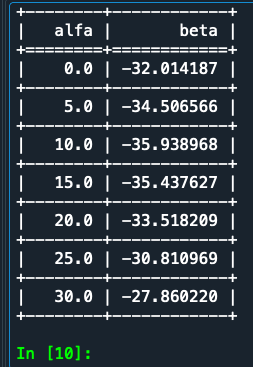
\includegraphics[scale=0.5]{Imagenes/diferenciacion_ejercicio_segmento_tabla.png}
\end{figure}
\end{frame}
\begin{frame}
\frametitle{Tabla completa de velocidad angular}
\begin{table}
\centering
\renewcommand{\arraystretch}{0.9}
\begin{tabular}{c | c}
$\alpha$ \, $[{}^{\circ}]$ & $\beta$ \, $[\SI{}{\radian\per\second}]$ \\ \hline
$0.0$ & $-32.014187$ \\ \hline
$5.0$ & $-34.506566$ \\ \hline
$10.0$ & $-35.938968$ \\ \hline
$15.0$ & $-35.437627$ \\ \hline
$20.0$ & $-33.518209$ \\ \hline
$25.0$ & $-30.810969$ \\ \hline
$30.0$ & $-27.860220$ \\ \hline
\end{tabular}
\end{table}
\end{frame}
\begin{frame}
\frametitle{Gráfica de la velocidad angular}
\begin{figure}
    \centering
    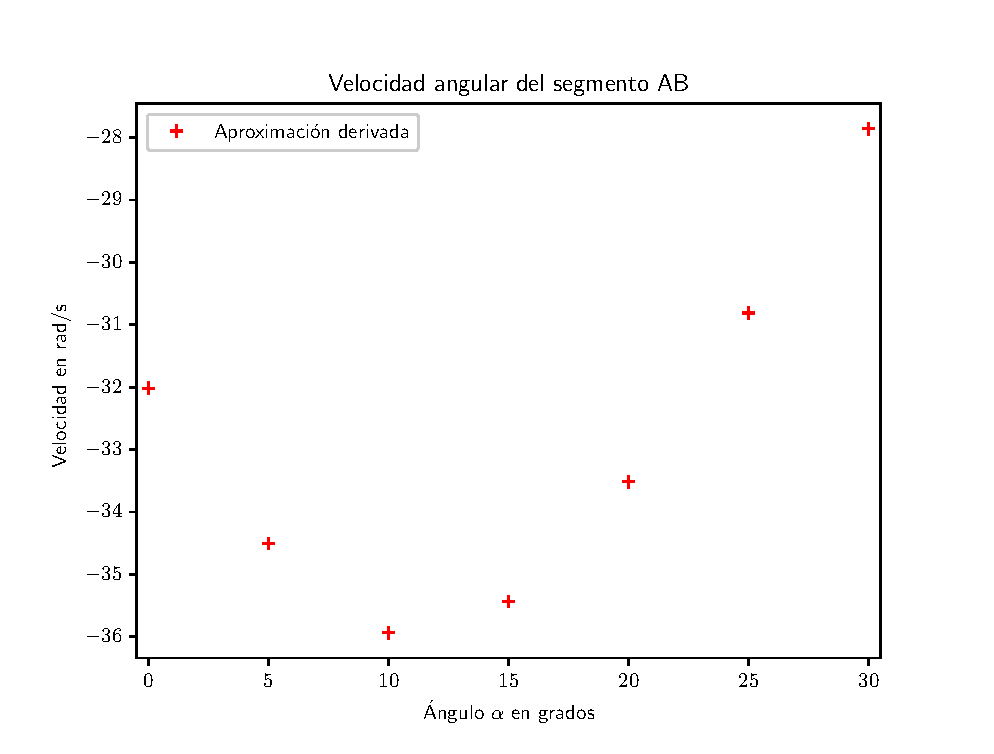
\includegraphics[scale=0.55]{Imagenes/diferenciacion_ejercicio_segmento_01.eps}
\end{figure}
\end{frame}
\begin{frame}
\frametitle{Ejercicio a cuenta}
Para practicar y repasar lo que hemos trabajado en este Tema 2, se te pide que entregues el código que genere la siguiente gráfica con una curva de de interpolación para la velocidad angular del segmento AB, con las funciones de \python.
\end{frame}
\begin{frame}
\frametitle{Sugerencias}
\setbeamercolor{item projected}{bg=black,fg=beige}
\setbeamertemplate{enumerate items}{%
\usebeamercolor[bg]{item projected}%
\raisebox{1.5pt}{\colorbox{bg}{\color{fg}\footnotesize\insertenumlabel}}%
}
\begin{enumerate}[<+->]
\item Sugerimos que obtengas más puntos de interpolación: $[2.5, 7.5, \ldots, 22.5, 27.5]$
\item Con esos nuevos puntos, obtén una curva de interpolación en el intervalo $[0.1, 29.9]$
\item Incluye una rutina de graficación.
\end{enumerate}
\end{frame}
\begin{frame}
\frametitle{Gráfica de interpolación de la velocidad angular}
\begin{figure}
    \centering
    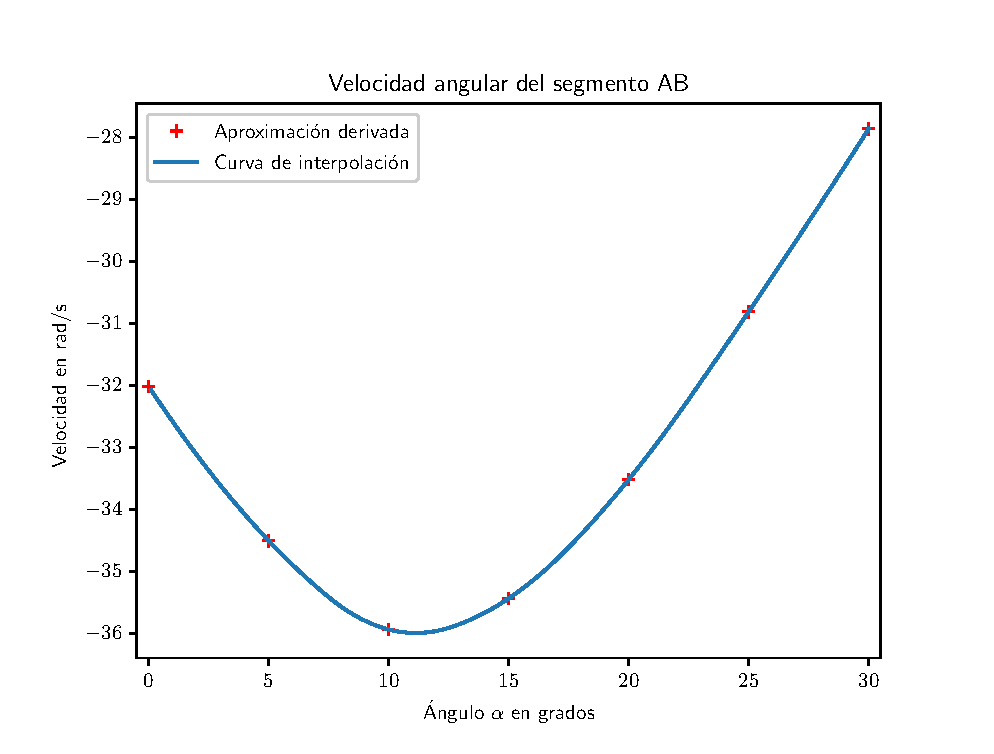
\includegraphics[scale=0.55]{Imagenes/diferenciacion_ejercicio_segmento_02.eps}
\end{figure}
\end{frame}
% \begin{frame}
% \frametitle{Ejercicio para entregar: Completa la tabla}
% \begin{center}
% \fontsize{12}{12}\selectfont
% \begin{tabular}{c | c | c | c | c | c | c | c}
% $\alpha$ (grados) & $0$ & $5$ & $10$ & $15$ & $20$ & $25$ & $30$  \\ \hline
% $\dot{\beta}$ (rad/s) & $-32.01$ & $-34.51$ &  &  &  &  & 
% \end{tabular}
% \end{center}
% \textcolor{red}{Debes de entregar la tabla y el código en \python.}
% \end{frame}
% %\begin{frame}
% %\frametitle{Ejercicio resuelto}
% %\begin{center}
% %\fontsize{12}{12}\selectfont
% %\begin{tabular}{c | c | c | c | c | c | c | c}
% %$\alpha$ (grados) & 0 & 5 & 10 & 15 & 20 & 25 & 30  \\ \hline
% %$\dot{\beta}$ (rad/s) & -32.01 & -34.51 & -35.94 & -35.44 & -33.52 & -30.81  & -27.86 
% %\end{tabular}
% %\end{center}
% %\textcolor{red}{Debe de entregarse la tabla y el código en python.}
% %\end{frame}

\section{Extrapolación de Richardson}
\frame{\tableofcontents[currentsection, hideothersubsections]}
\subsection{Definición}

\begin{frame}
\frametitle{Extrapolación de Richardson}
La Extrapolación de Richardson es un método sencillo para aumentar la precisión de ciertos procedimientos numéricos, incluyendo las aproximaciones por diferencias finitas.
\\
\bigskip
\pause
Supongamos que tenemos la forma de calcular una cantidad $G$. Por otra parte, si consideramos que el resultado depende de un parámetro $h$, hagamos la aproximación por $g (h)$, tenemos que $G = g (h) + E (h)$, donde $E (h)$ representa el error.
\end{frame}
% \begin{frame}
% La extrapolación de Richardson puede remover el error, siempre que tenga la forma $E(h) = ch^{p}$, donde $c$ y $p$ son constantes. Iniciamos el cálculo para varios valores de $h$, digamos $h=h_{1}$, así
% \[ G = g(h_{1}) + c h_{1}^{p}\]
% Repetimos el cálculo con $h=h_{2}$, por tanto:
% \[ G = g(h_{2}) + c h_{2}^{p} \]
% \end{frame}
% \begin{frame}
% Eliminando $c$ y resolviendo para $G$, tenemos:
% \[ G = \dfrac{(h_{1}/h_{2})^{p} g(h_{2}) - g(h_{1})}{(h_{1}/h_{2})^{p}-1}\]
% que es la fórmula de Extrapolación de Richardson. En la práctica se usa $h_{2} = h_{1}/2$, quedando
% \[ G = \dfrac{2^{p} g(h_{1}/2) - g(h_{1})}{2^{p}-1}\]
% \end{frame}
% \begin{frame}
% \frametitle{Ejemplo}
% Usemos el ejemplo de $(exp(-x))''$ en $x=1$, consideremos los valores de la tabla con seis dígitos.
% \\
% \bigskip
% Dado que la extrapolación contine errores por truncamiento, debemos limitarnos a los valores de $h$ que producen redondeo insignificante.
% \end{frame}
% \begin{frame}
% De la tabla anterior que calculamos, tenemos que:
% \[ g(0.64) = 0.380609 \hspace{2cm} g(0.32) = 0.371029\]
% El error de truncamiento en la aproximación central por diferencias finitas es:
% \[E(h) = O(h^{2}) = c_{1}h^{2} + c_{2}h^{4} + c_{3}h^{6} + \ldots\]
% \end{frame}
% \begin{frame}
% Por lo que podemos eliminar el primer término del error (dominante), si usamos $p=2$ y $h_{1}=0.64$, así
% \[ \begin{split}
% G =& \dfrac{2^{2}g(0.32)- g(0.64}{2^{2}-1} = \dfrac{4(0.371035)-0.380610}{3} \\
%  =& 0.367843
% \end{split} \]
% Que es una aproximación de $(exp(-x))''$ con un error $=O(h^{4})$. Que es el mejor valor obtenido en comparación de los obtenidos con precisión de ocho dígitos.
% \end{frame}
% \begin{frame}
% \frametitle{Ejemplo}
% Teniendo en cuenta los puntos de datos uniformemente espaciados:
% \begin{center}
% \begin{tabular}{c | c | c | c | c | c }
% x & $0$ & $0.1$ & $0.2$ & $0.3$ & $0.4$ \\ \hline
% f(x) & $0.0000$ & $0.0819$ & $0.1341$ & $0.1646$ & $0.1797$
% \end{tabular}
% \end{center}
% Calcular $f'(x)$ y $f''(x)$ en $x=0$ y $x=0.2$, usando la aproximación por diferencias finitas de orden $O(h^{2})$.
% \end{frame}
% \begin{frame}
% \frametitle{Solución}
% Usando la aproximación por diferencias finitas de orden $O(h^{2})$, de la lista de diferencias hacia adelante, tenemos:
% \[ \begin{split} 
% f'(0) =& \dfrac{-3f(0) + 4f(0.1) - f(0.2)}{2(0.1)} = 0.967 \\
% f''(0) =& \dfrac{2 f(0) - 5f(0.1) + 4f(0.2) - f(0.3)}{(0.1)^{2}} = -3.77
% \end{split} \]
% \end{frame}
% \begin{frame}
% Si usamos ahora la aproximación por diferencias centrales:
% \[ \begin{split}
% f'(0.2) =& \dfrac{-f(0.1) + f(0.3)}{2(0.1)} = 0.4135 \\
% f''(0.2) =& \dfrac{f(0.1)-2f(0.2) + f(0.3)}{(0.1)^{2}} = -2.17
% \end{split} \]
% \end{frame}
% \begin{frame}
% \frametitle{Otro Ejemplo}
% Usando los siguientes datos(del ejemplo anterior):
% \begin{center}
% \begin{tabular}{c | c | c | c | c | c }
% x & $0$ & $0.1$ & $0.2$ & $0.3$ & $0.4$ \\ \hline
% f(x) & $0.0000$ & $0.0819$ & $0.1341$ & $0.1646$ & $0.1797$
% \end{tabular}
% \end{center}
% Calcular $f'(0)$ con la mayor precisión posible.
% \\
% \medskip
% Una solución es usar el método de extrapolación de Richardson con aproximación de diferencias finitas.
% \end{frame}
% \begin{frame}
% \frametitle{Solución}
% Iniciamos con la segunda aproximación por diferencias hacia adelante de orden $O(h^{2})$ para $f'(0)$: usamos en una $h=0.2$ y en otra $h=0.1$
% \[ \begin{split}
% g(0.2) =& \dfrac{-3f(0) + 4f(0.2) - f(0.4)}{2(0.2)} = 0.8918 \\
% g(0.1) =& \dfrac{-3f(0) + 4f(0.1) - f(0.2)}{2(0.1)} = 0.9675
% \end{split} \]
% Recordemos que el error en ambas aproximaciones, es de la forma $E(h) = c_{1}h^{2} + c_{2} h^{4} + c_{3}h^{5} + \ldots$. 
% \end{frame}
% \begin{frame}
% Usamos la extrapolación de Richardson para eliminar el término dominante. Con $p=2$, resulta
% \[ f'(0) \simeq G = \dfrac{2^{2}g(0.1)-g(0.2)}{2^{2}-1}=0.9927 \]
% la cual es una aproximación por diferencias finitas de orden $O(h^{4})$.
% \end{frame}
\end{document}
